    \begin{subfigure}[b]{0.33\textwidth}
    \centering
    \resizebox{\textwidth}{!}{
    \begin{tikzpicture}
    % learn
    \node at (0, 1.8) {\footnotesize ``This is a {\color{borange} dax}''};    
    \node at (0, 1) {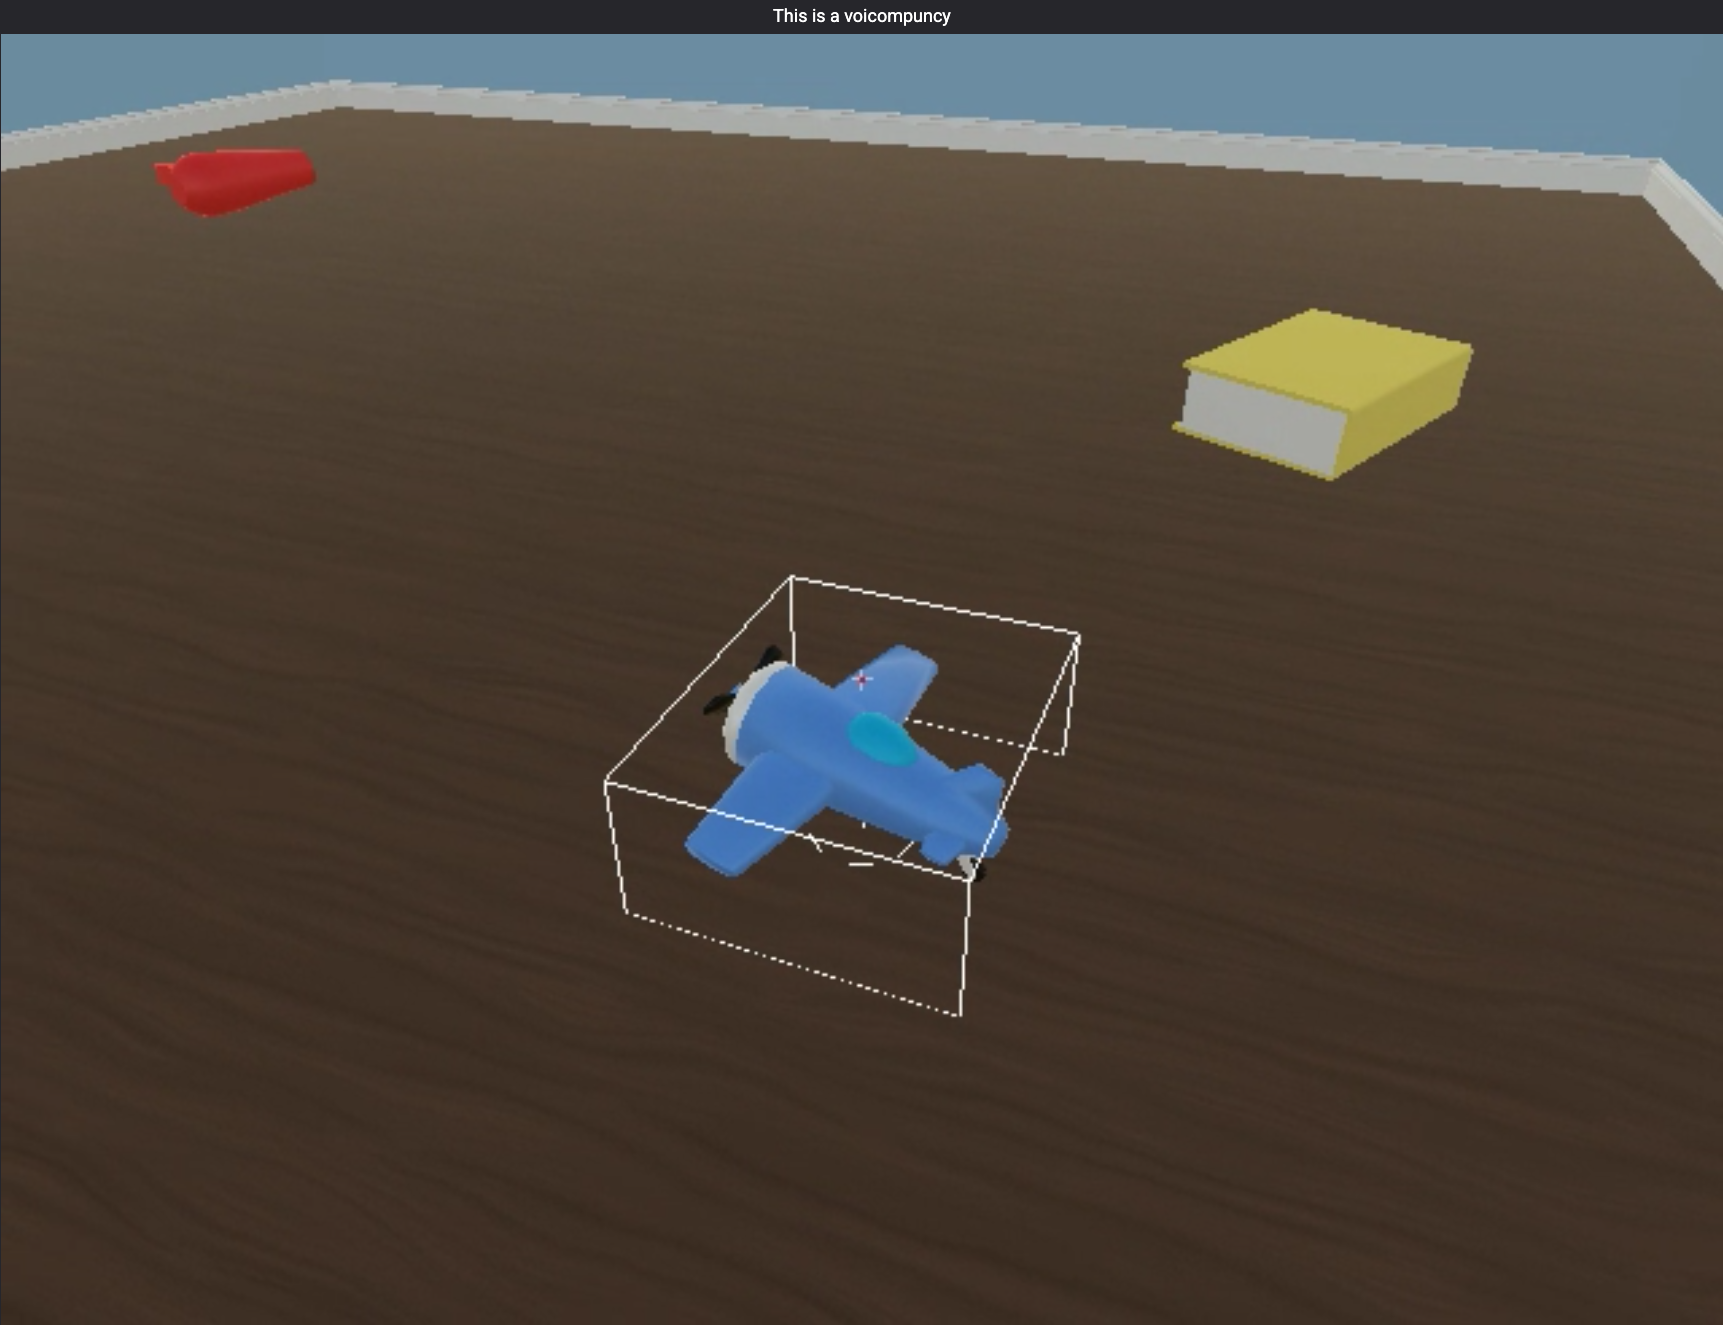
\includegraphics[width=1.5cm]{figures/task_images/fast_binding/binding.png}};
    \path [annobrace] (-0.75, 0.33) -- (0.75, 0.33) node [annotext] {\footnotesize Learn 3 new words};
    %distract
    \node at (2, 1.8) {\footnotesize ``Lift a rocket''};    
    \node at (2, 1) {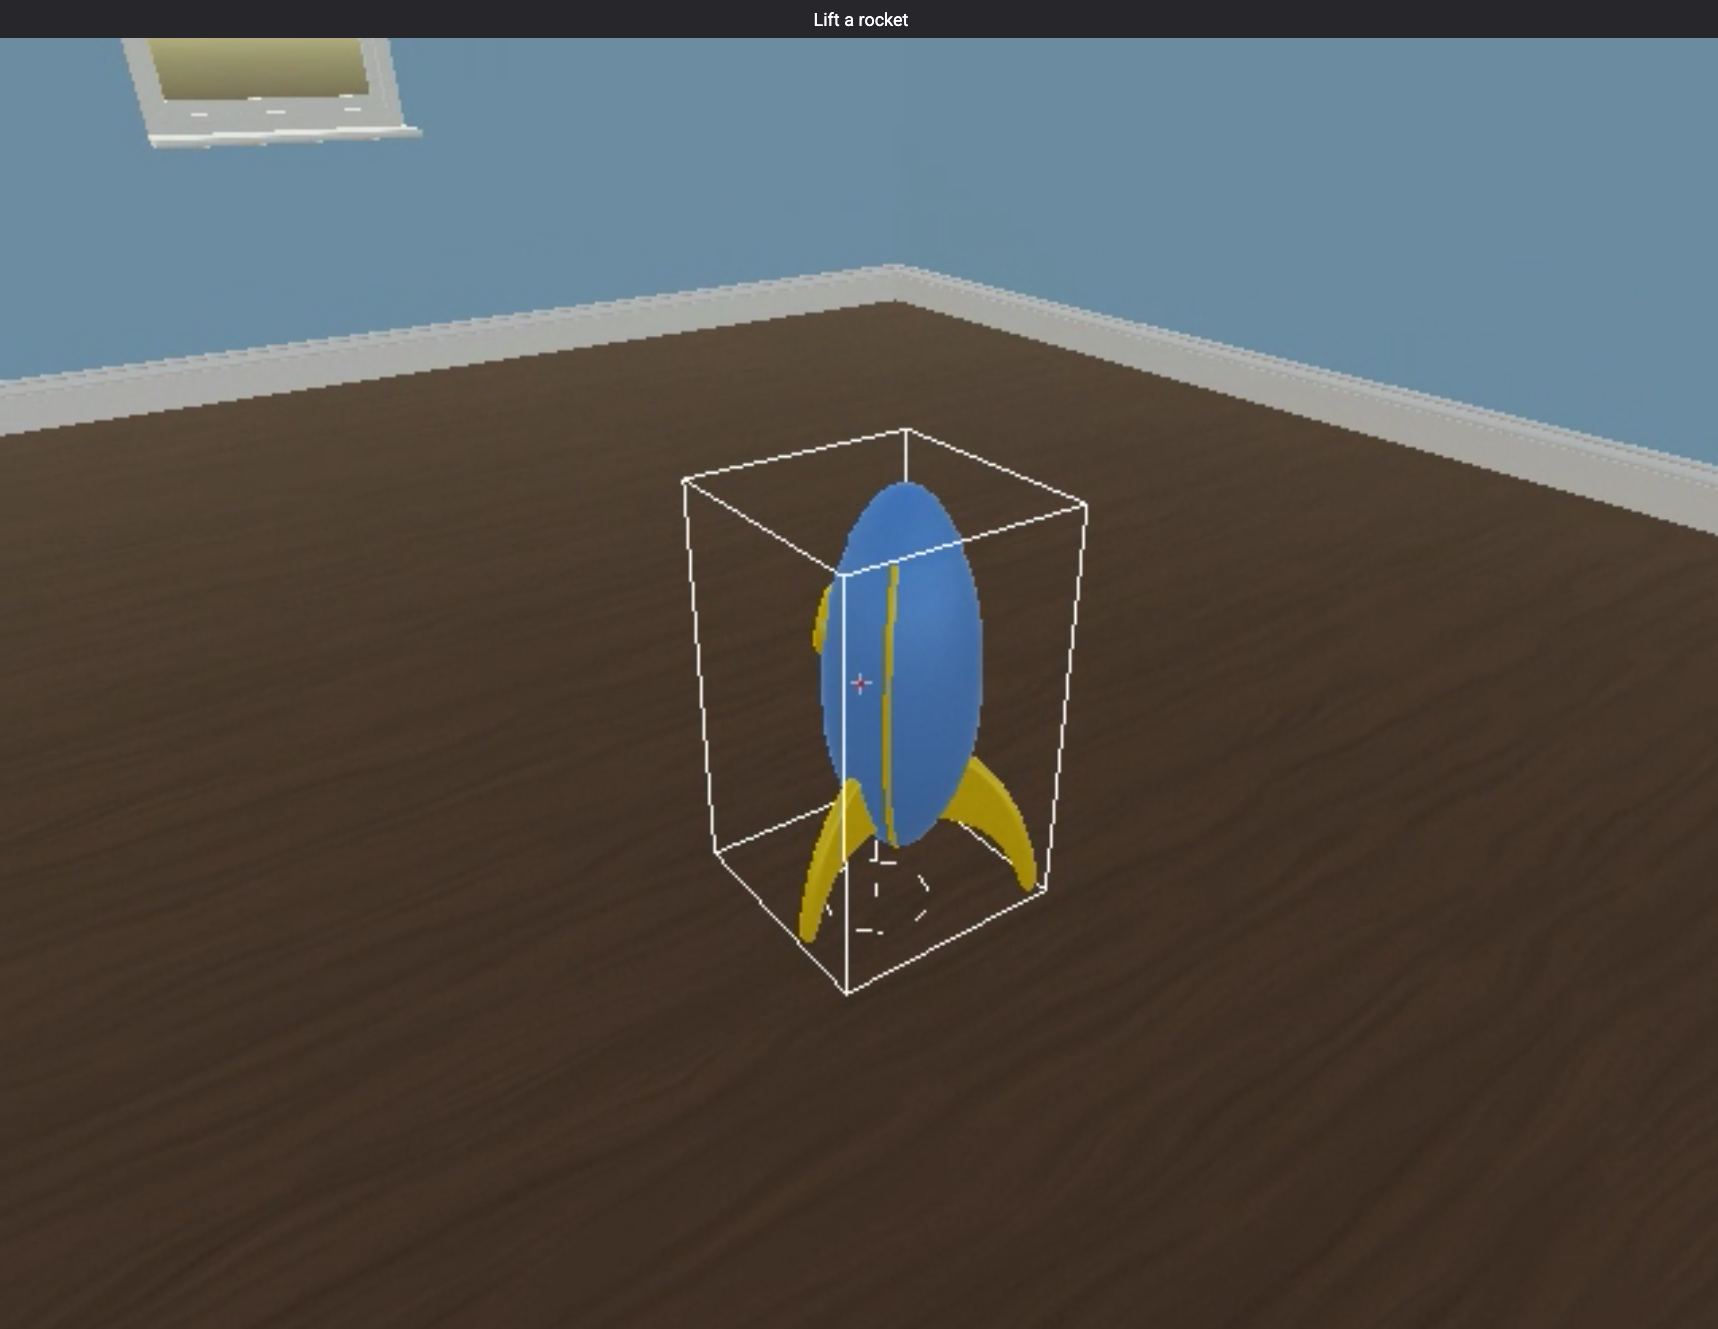
\includegraphics[width=1.5cm]{figures/task_images/fast_binding/distractor.png}};
    \path [annobrace] (1.25, 0.33) -- (2.75, 0.33) node [annotext] {\footnotesize Distractor tasks\! (\(N\times\))};
    % test
    \node at (4, 1.8) {\footnotesize ``Find a {\color{borange}dax}''};    
    \node at (4, 1) {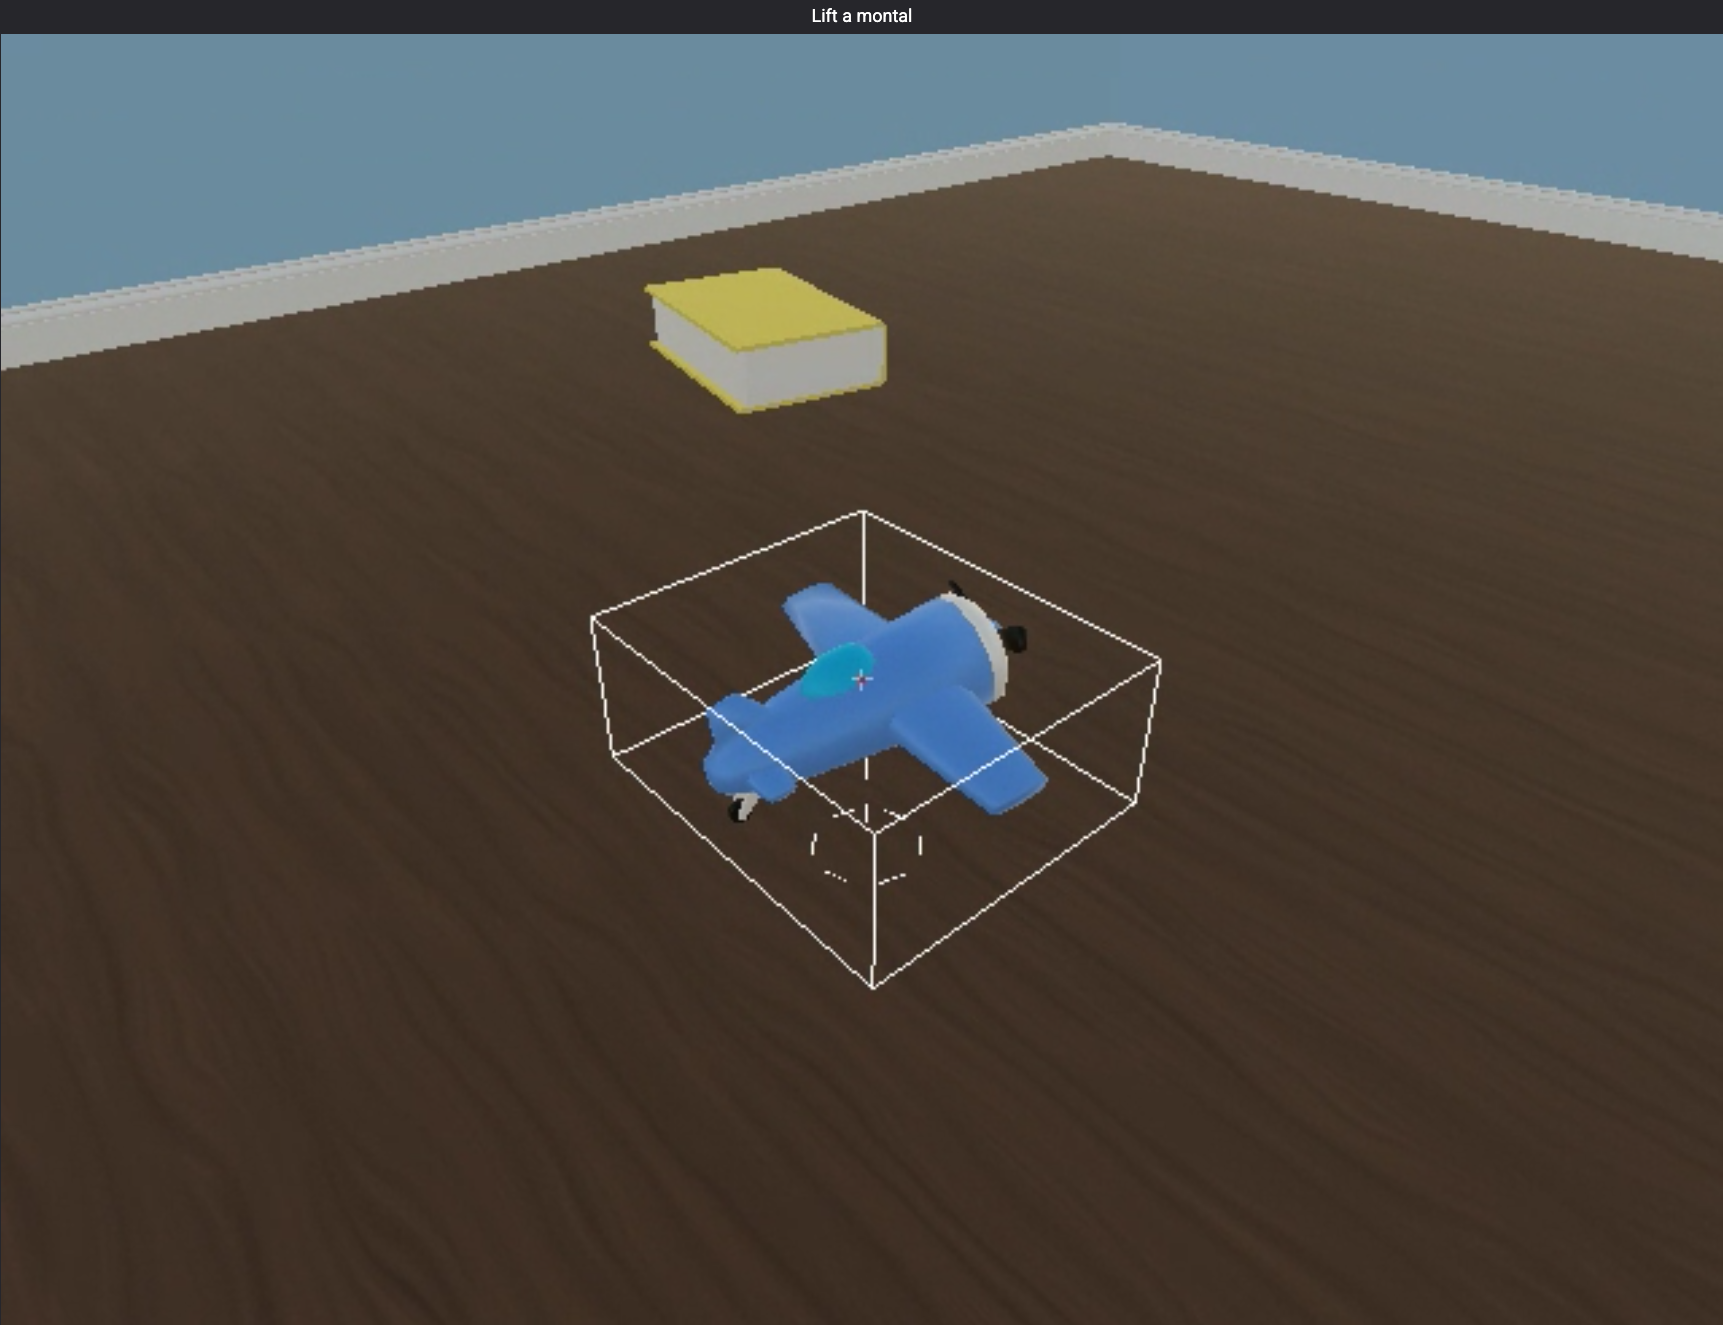
\includegraphics[width=1.5cm]{figures/task_images/fast_binding/testing.png}};
    \path [annobrace] (3.25, 0.33) -- (4.75, 0.33) node [annotext] {\footnotesize Test word recall};
    \path [arrow, very thick, borange, bend right=20] (4.3, 2) to (0.75, 2);
    \end{tikzpicture}
    }
%    \vspace{2.65cm}
    \captionsetup{width=.8\textwidth}
    \caption{Rapid word-learning with distractor tasks.} \label{fig:exp:fast_binding_tasks:distractors}
    \end{subfigure}%
    \begin{subfigure}[b]{0.33\textwidth}
    \centering
    \resizebox{\textwidth}{!}{
    \begin{tikzpicture}
    % learn
    \node at (0, 1.6) {\footnotesize ``This is a {\color{borange} dax}''};    
    \node at (0, 0.8) {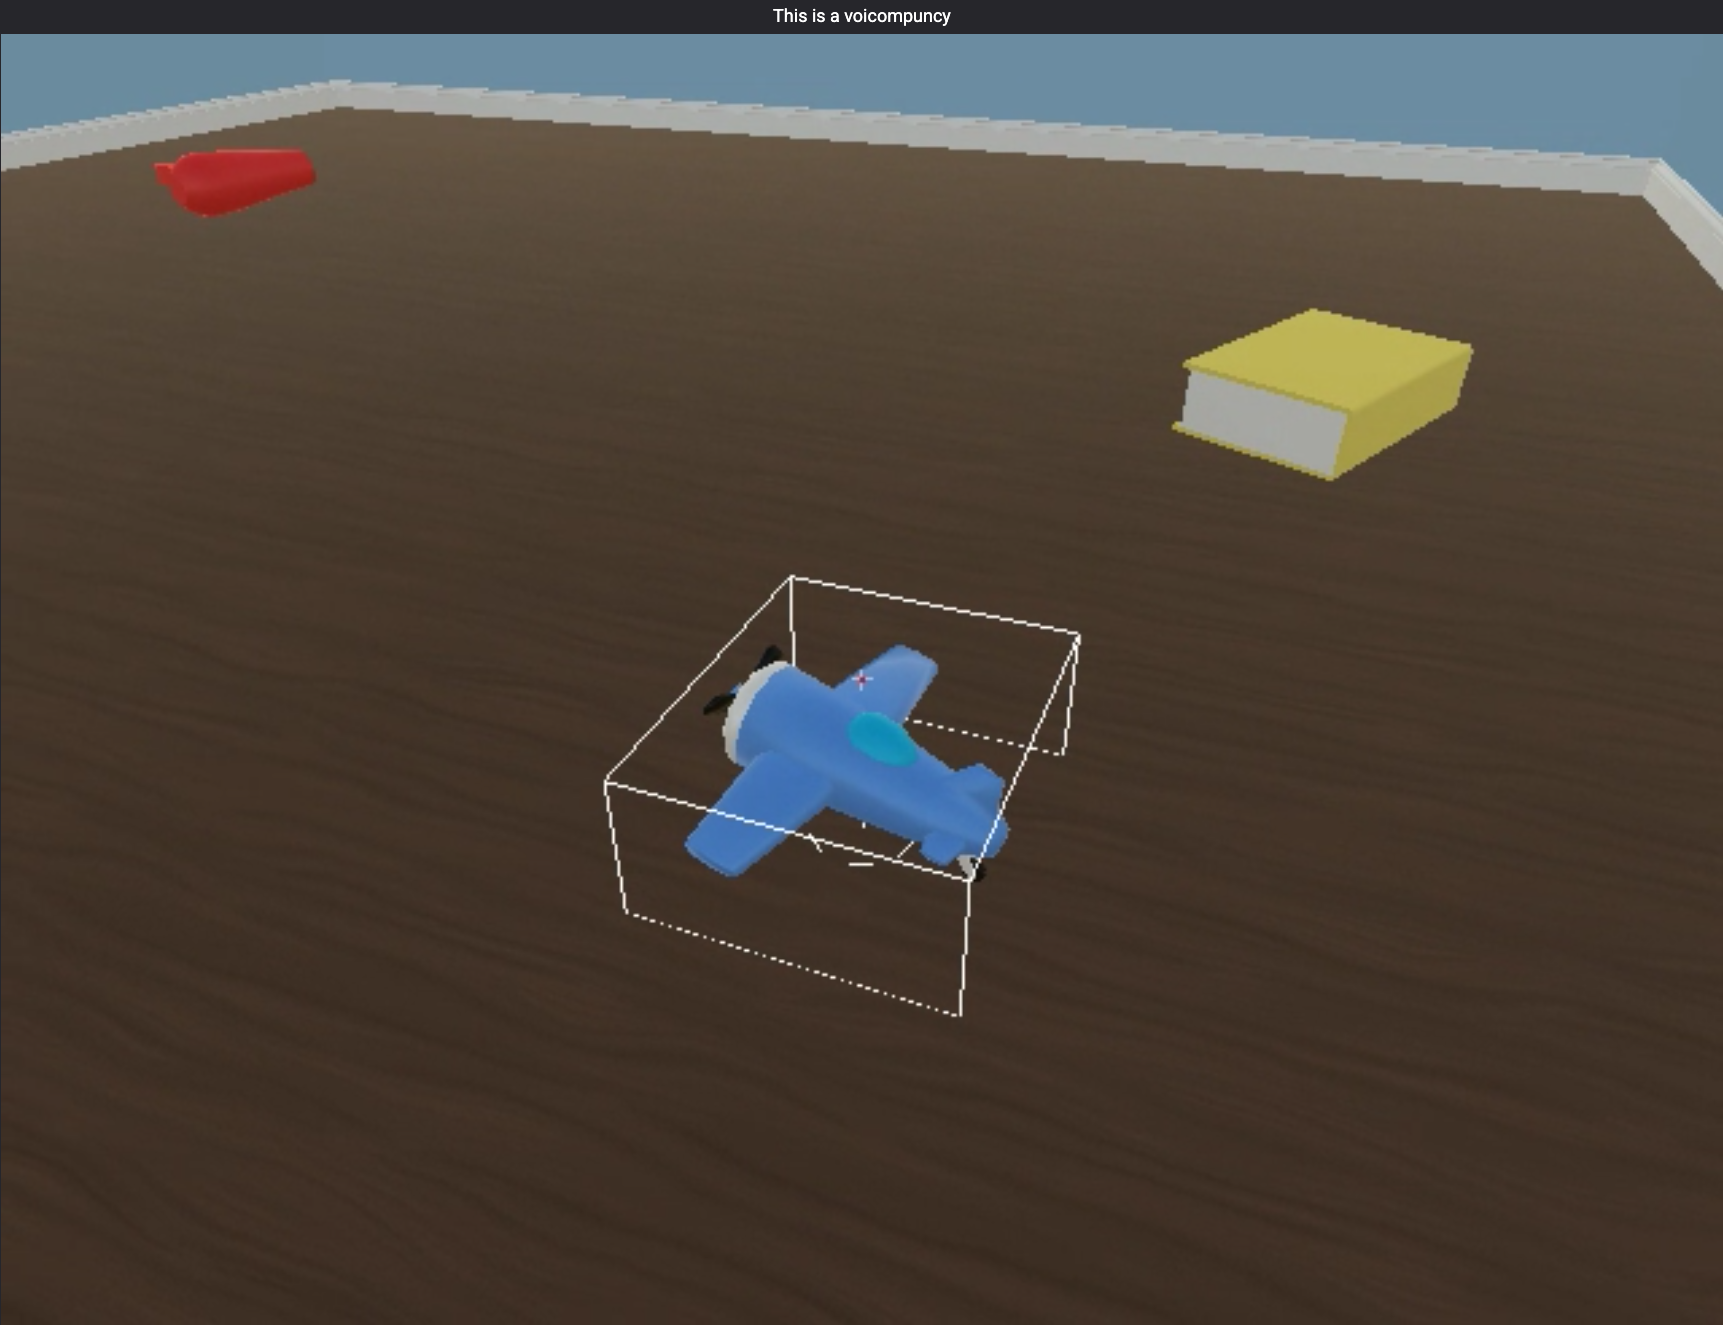
\includegraphics[width=1.5cm]{figures/task_images/fast_binding/binding.png}};
    \path [annobrace] (-0.75, 0.13) -- (0.75, 0.13) node [annotext] {\footnotesize Learn};
    %distract
    \node at (2, 1.6) {\footnotesize ``Lift a rocket''};    
    \node at (2, 0.8) {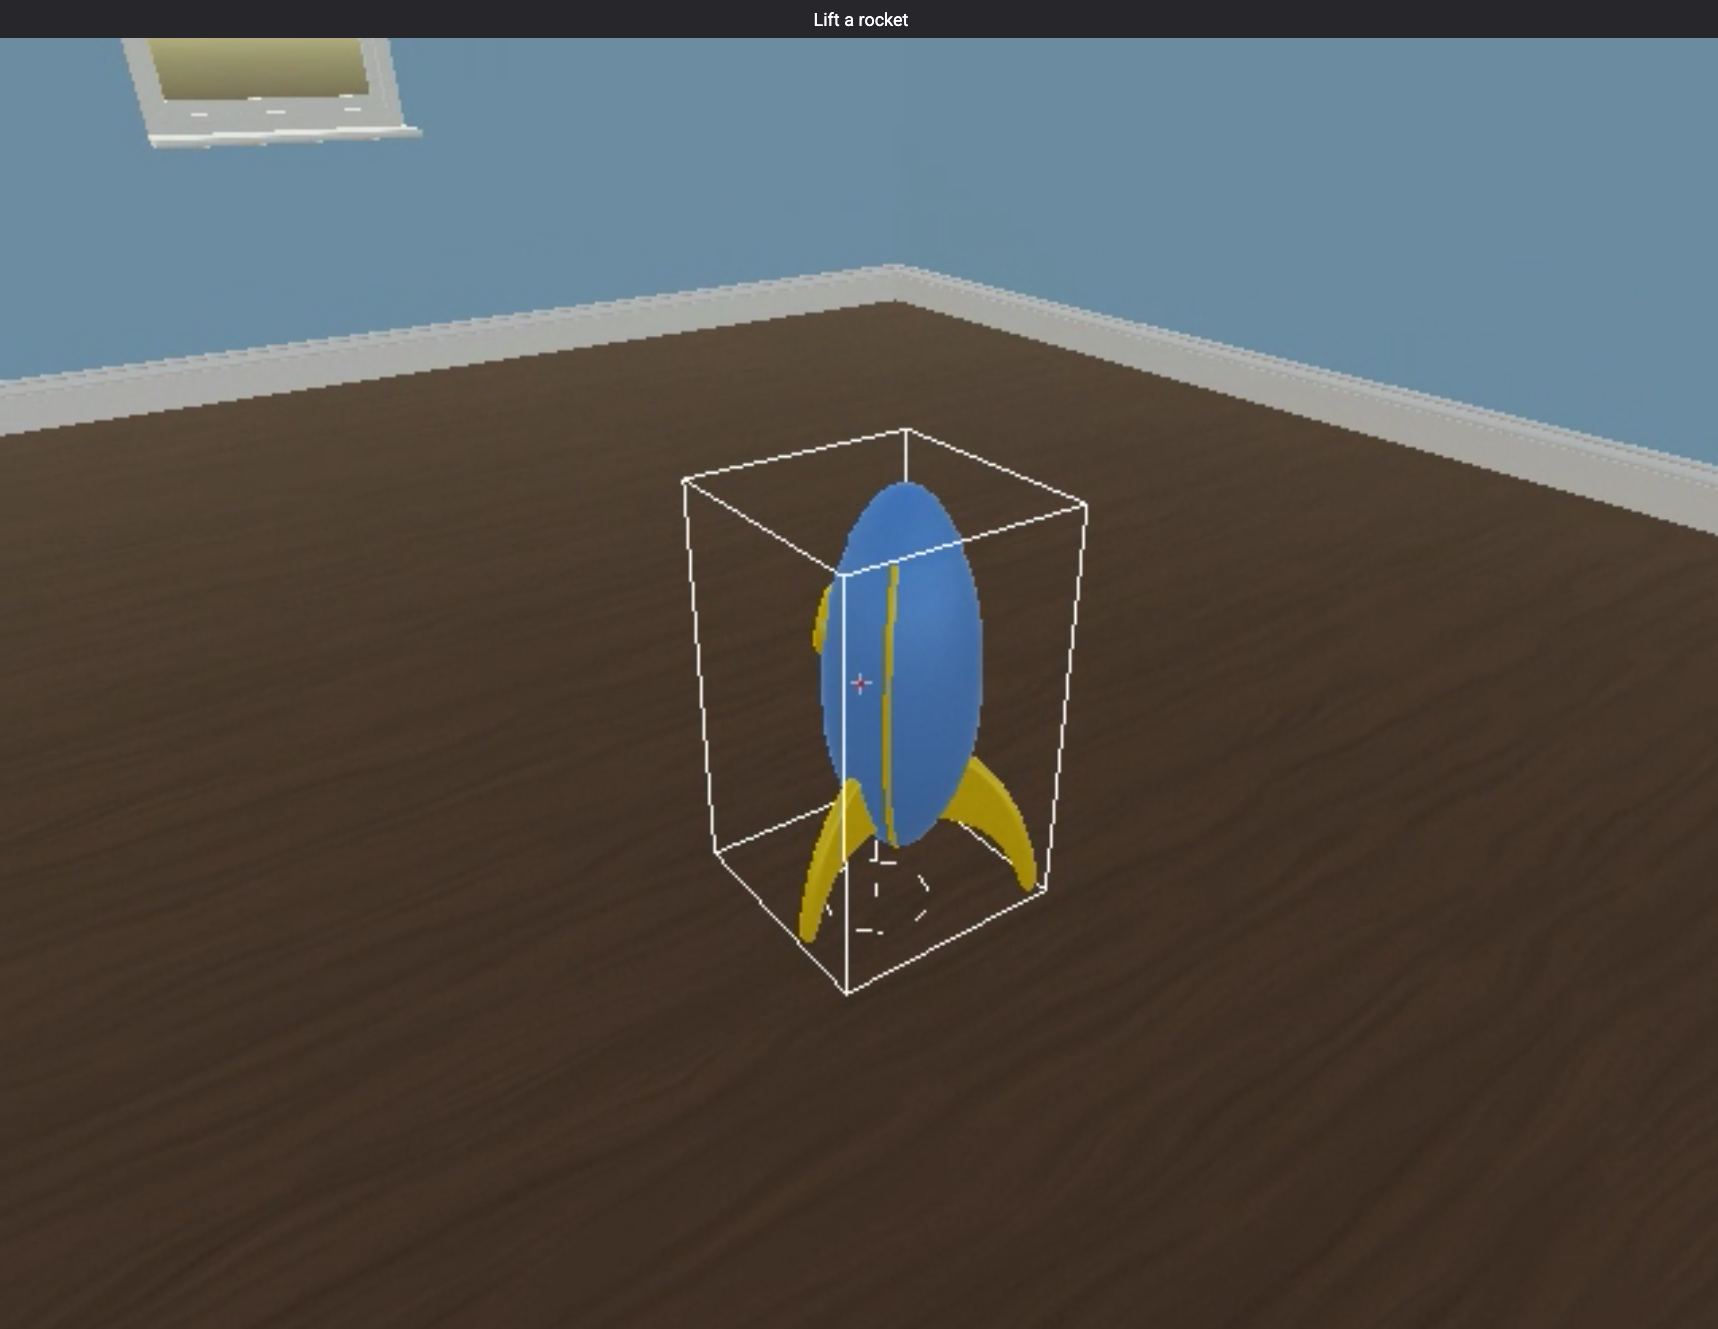
\includegraphics[width=1.5cm]{figures/task_images/fast_binding/distractor.png}};
    \path [annobrace] (1.25, 0.13) -- (2.75, 0.13) node [annotext] {\footnotesize Distractors};
    % test
    \node at (4, 1.6) {\footnotesize ``Find a {\color{bgreen}zipf}''};    
    \node at (4, 0.8) {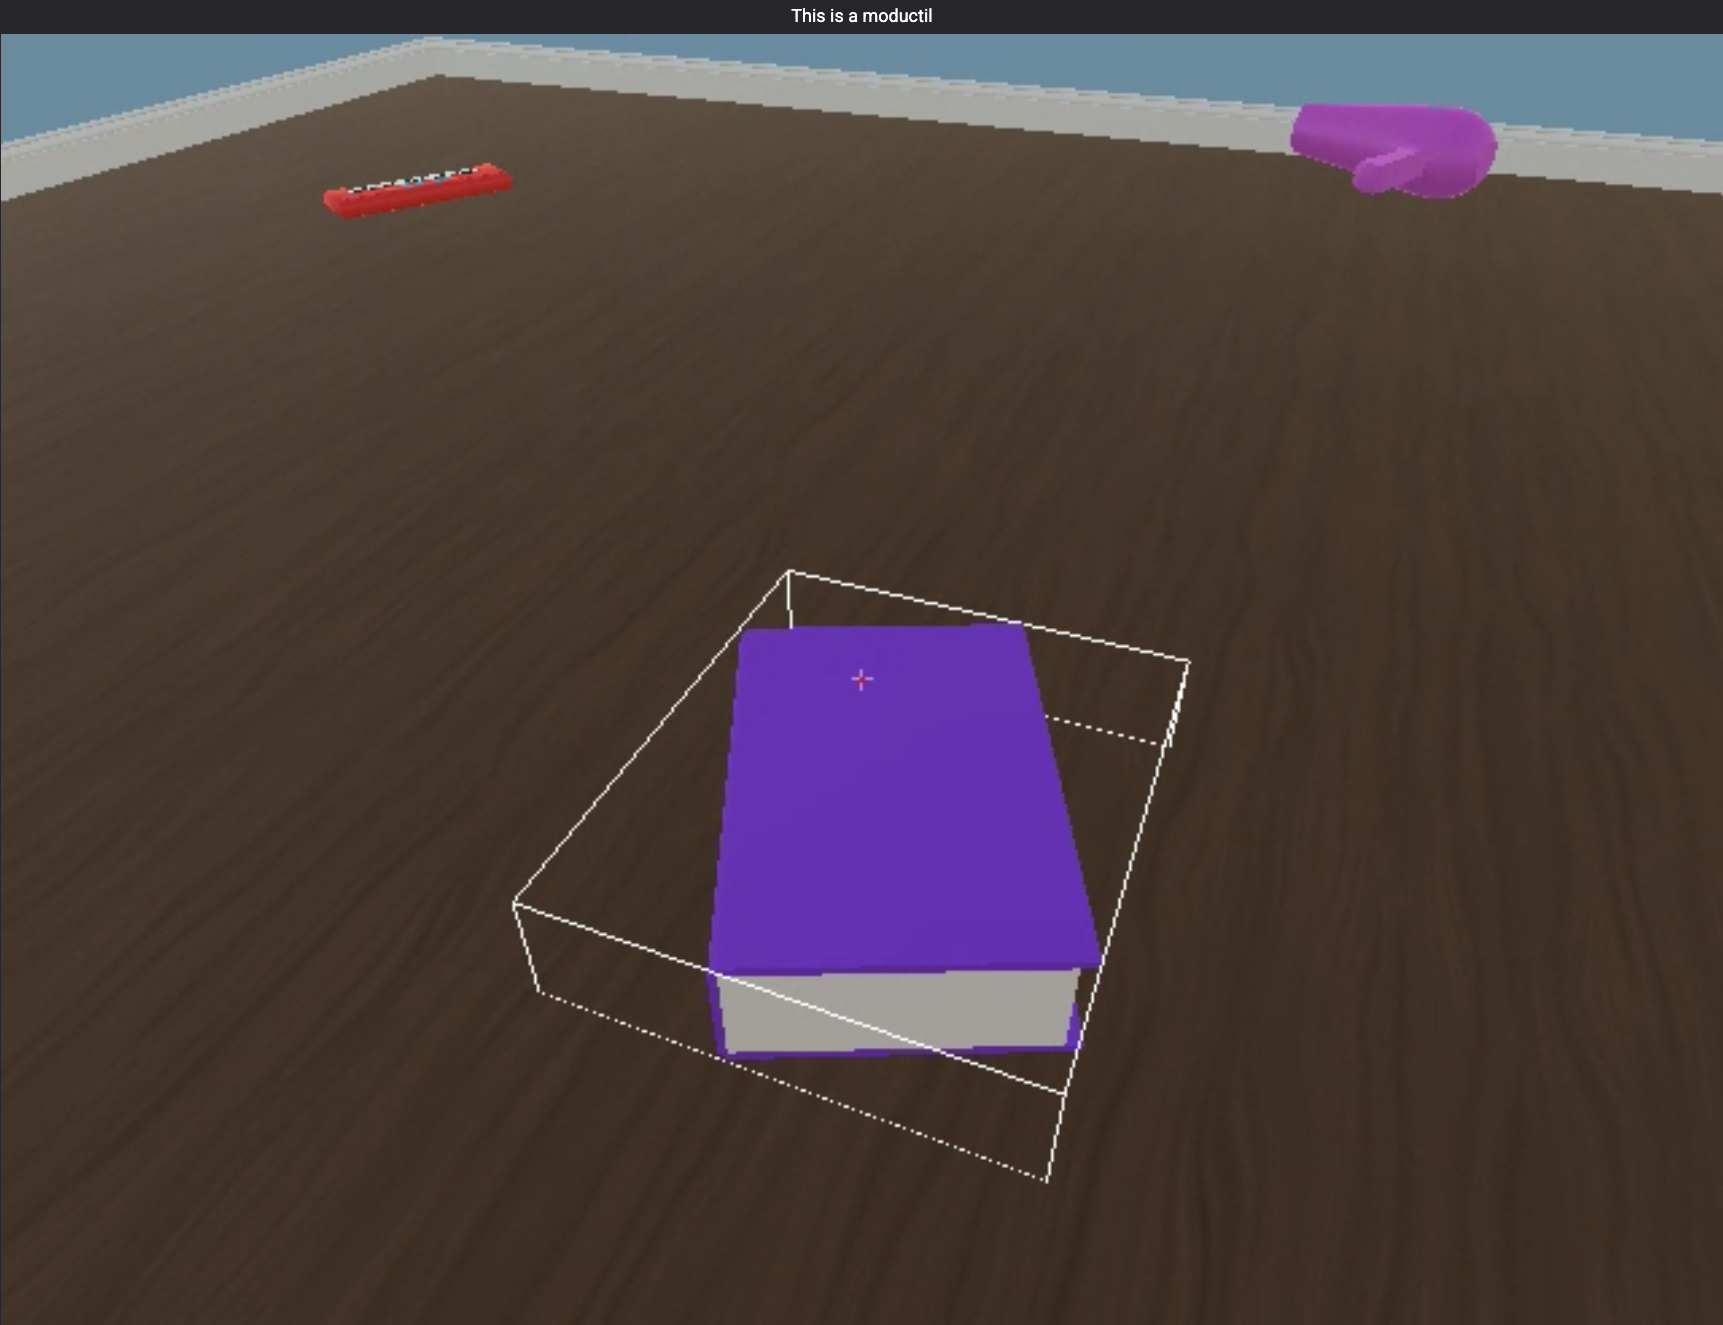
\includegraphics[width=1.5cm]{figures/task_images/fast_binding/testing2.png}};
    \path [annobrace] (3.25, 0.13) -- (4.75, 0.13) node [annotext] {\footnotesize Test};
    
    \node [scale=1.7] at (2, -0.55) {\large \(\vdots\)};
    
    \begin{scope}[shift={(0, -3)}]
    \node at (0, 1.8) {\footnotesize ``This is a {\color{bpurp} zark}''};    
    \node at (0, 1) {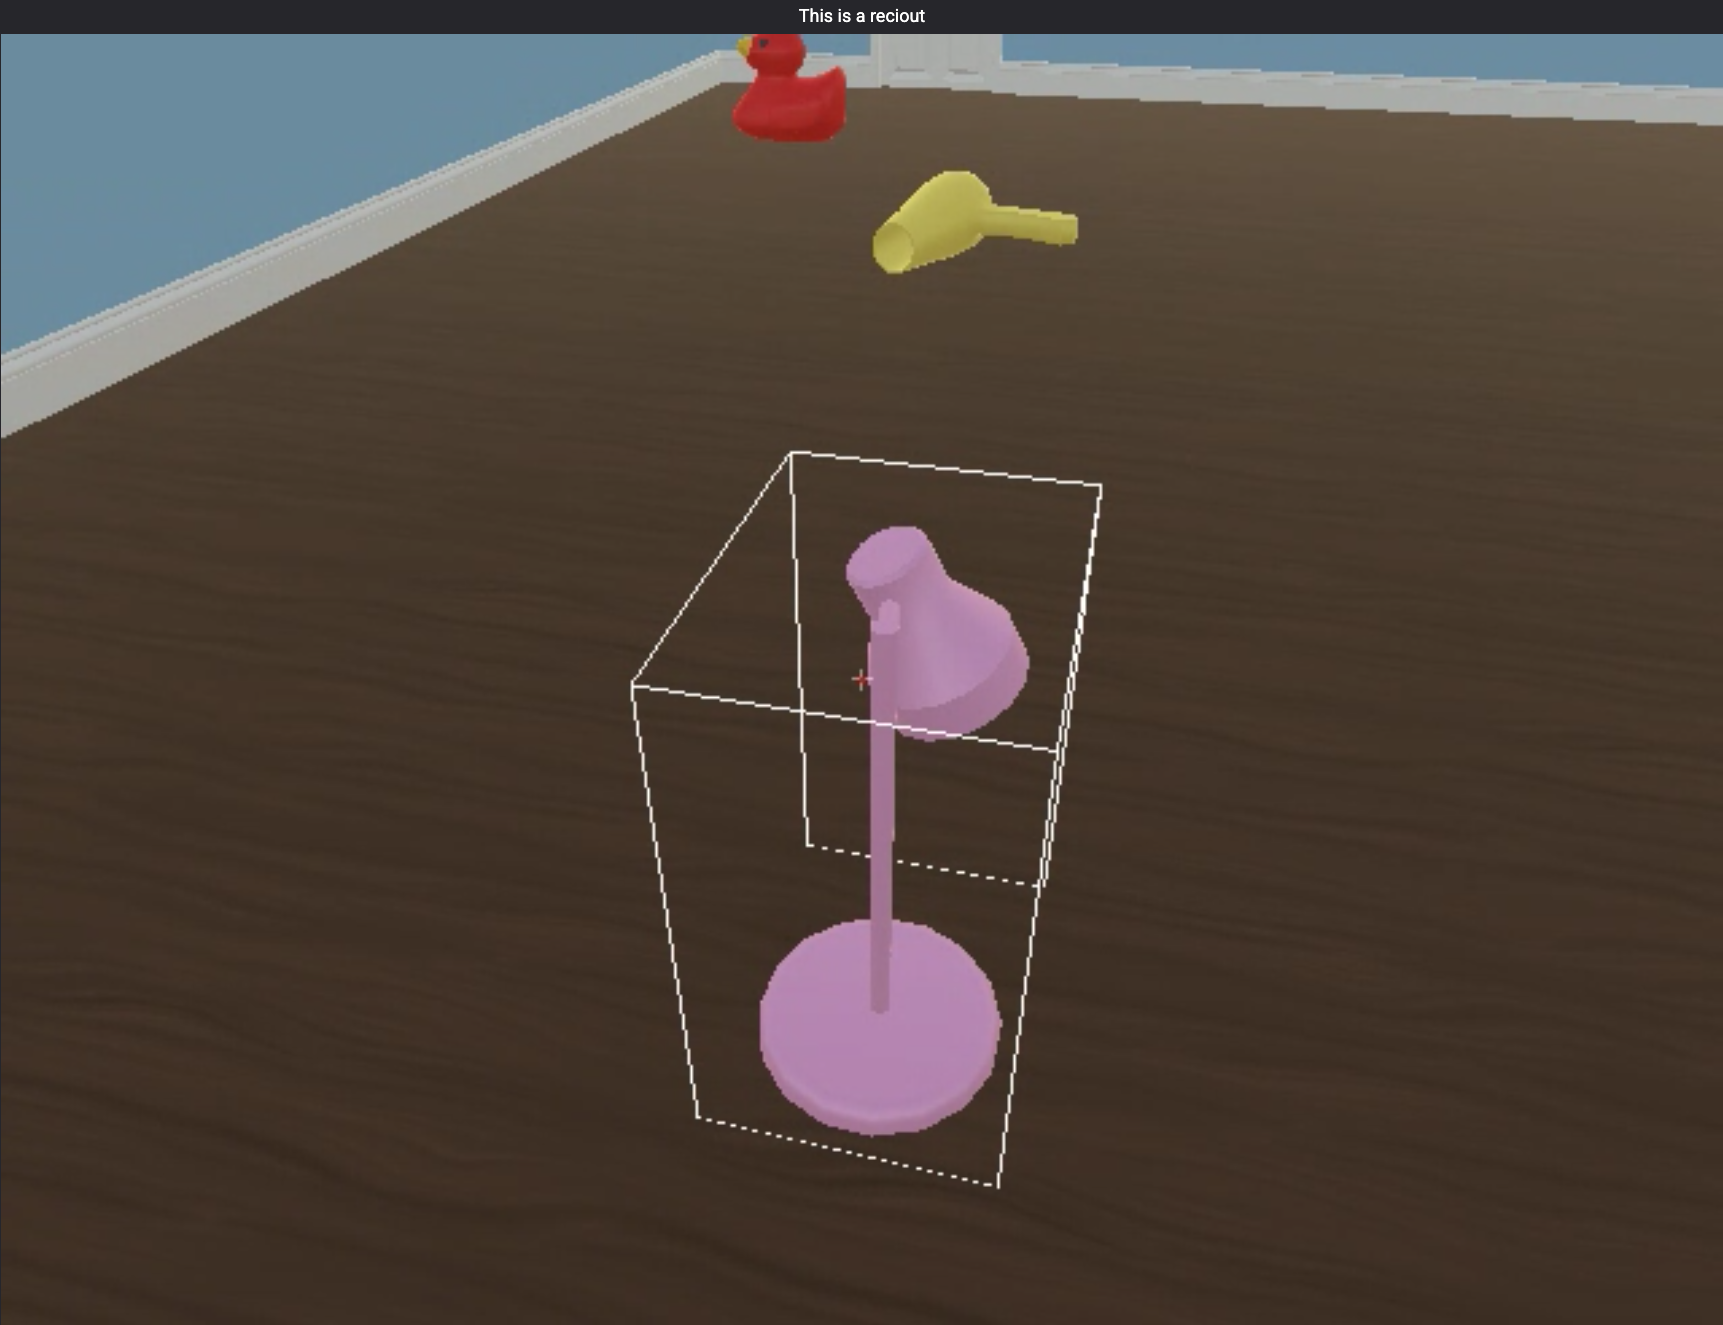
\includegraphics[width=1.5cm]{figures/task_images/fast_binding/binding2.png}};
    \path [annobrace] (-0.75, 0.33) -- (0.75, 0.33) node [annotext] {\footnotesize Learn};
    %distract
    \node at (2, 1.8) {\footnotesize ``Lift a train''};    
    \node at (2, 1) {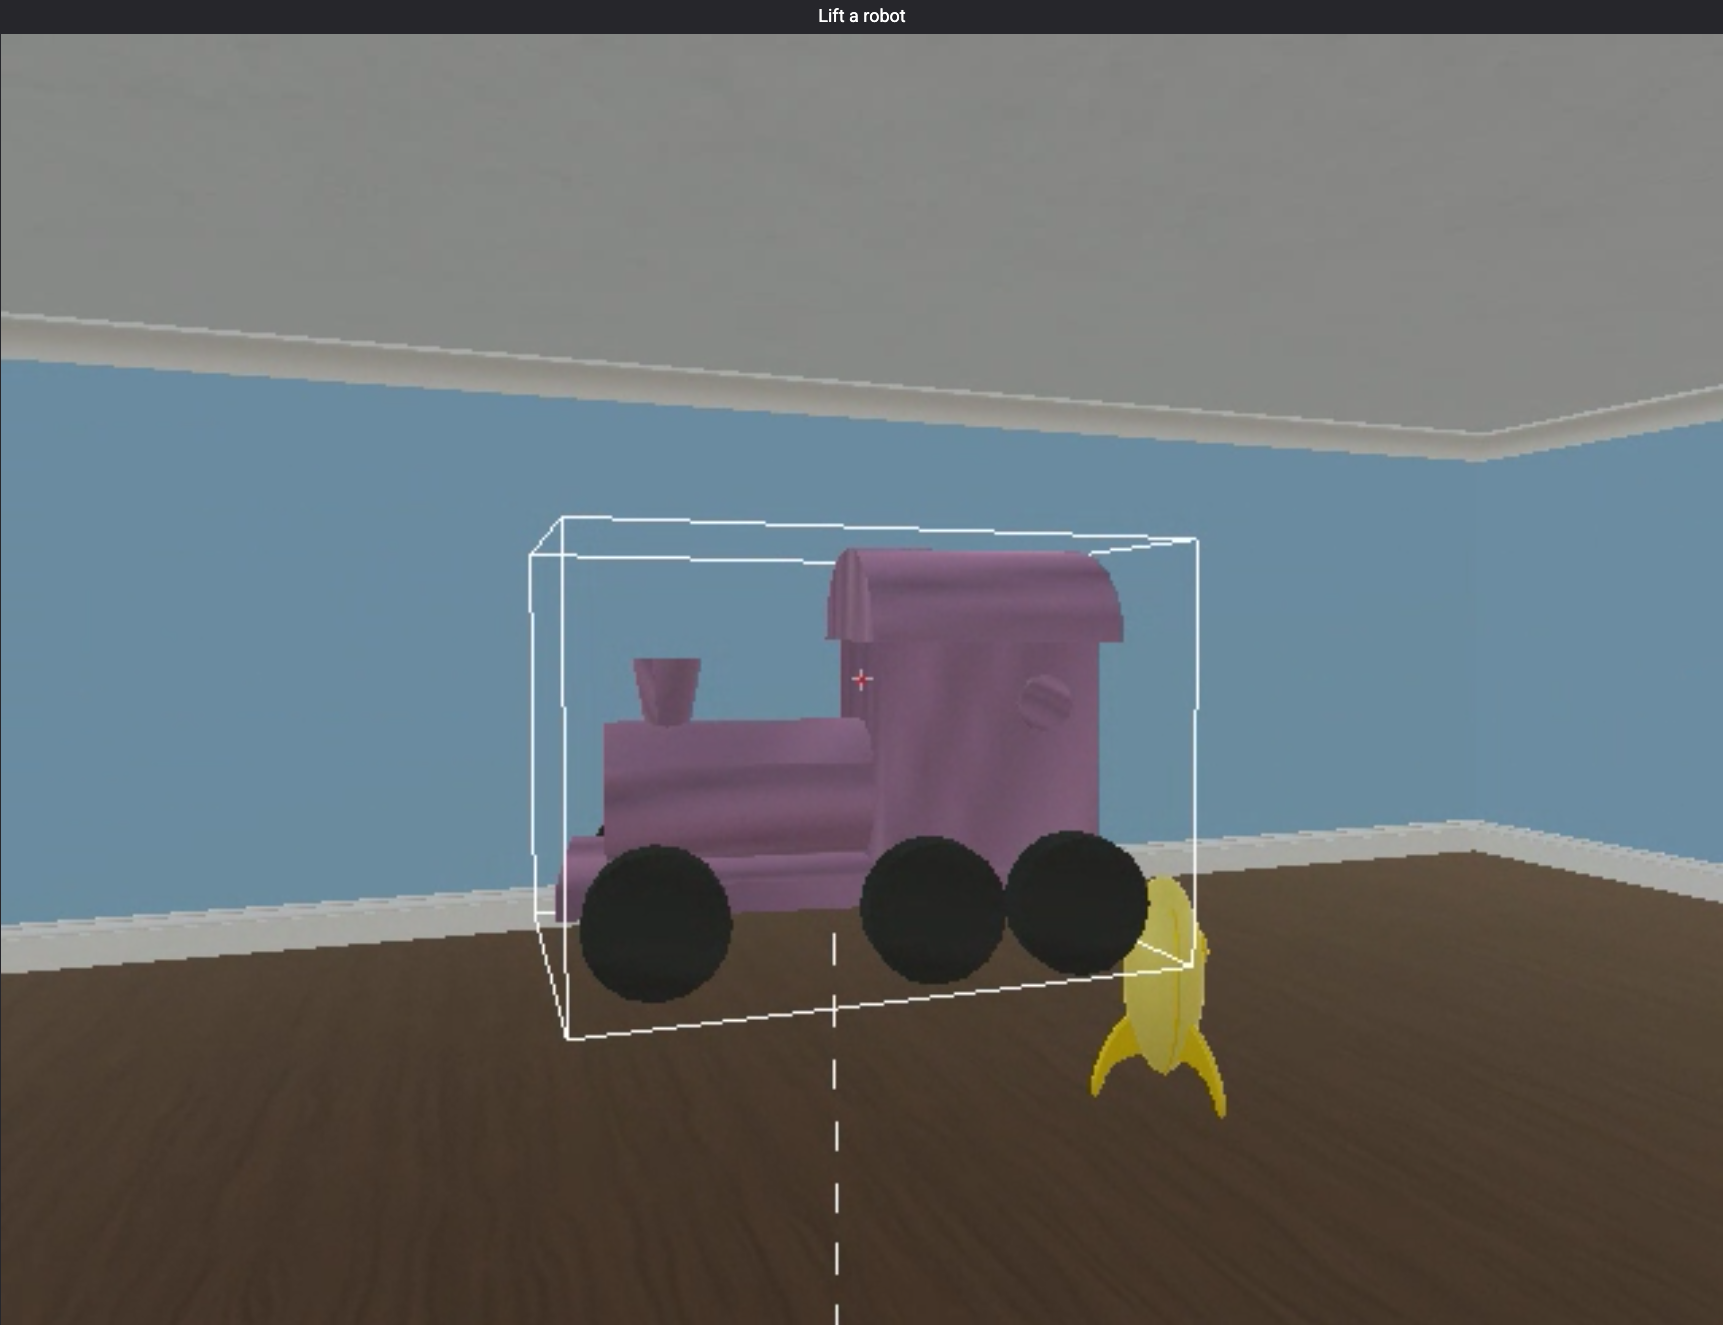
\includegraphics[width=1.5cm]{figures/task_images/fast_binding/distractor2.png}};
    \path [annobrace] (1.25, 0.33) -- (2.75, 0.33) node [annotext] {\footnotesize Distractors};
    % test
    \node at (4, 1.8) {\footnotesize ``Find a {\color{borange}dax}''};    
    \node at (4, 1) {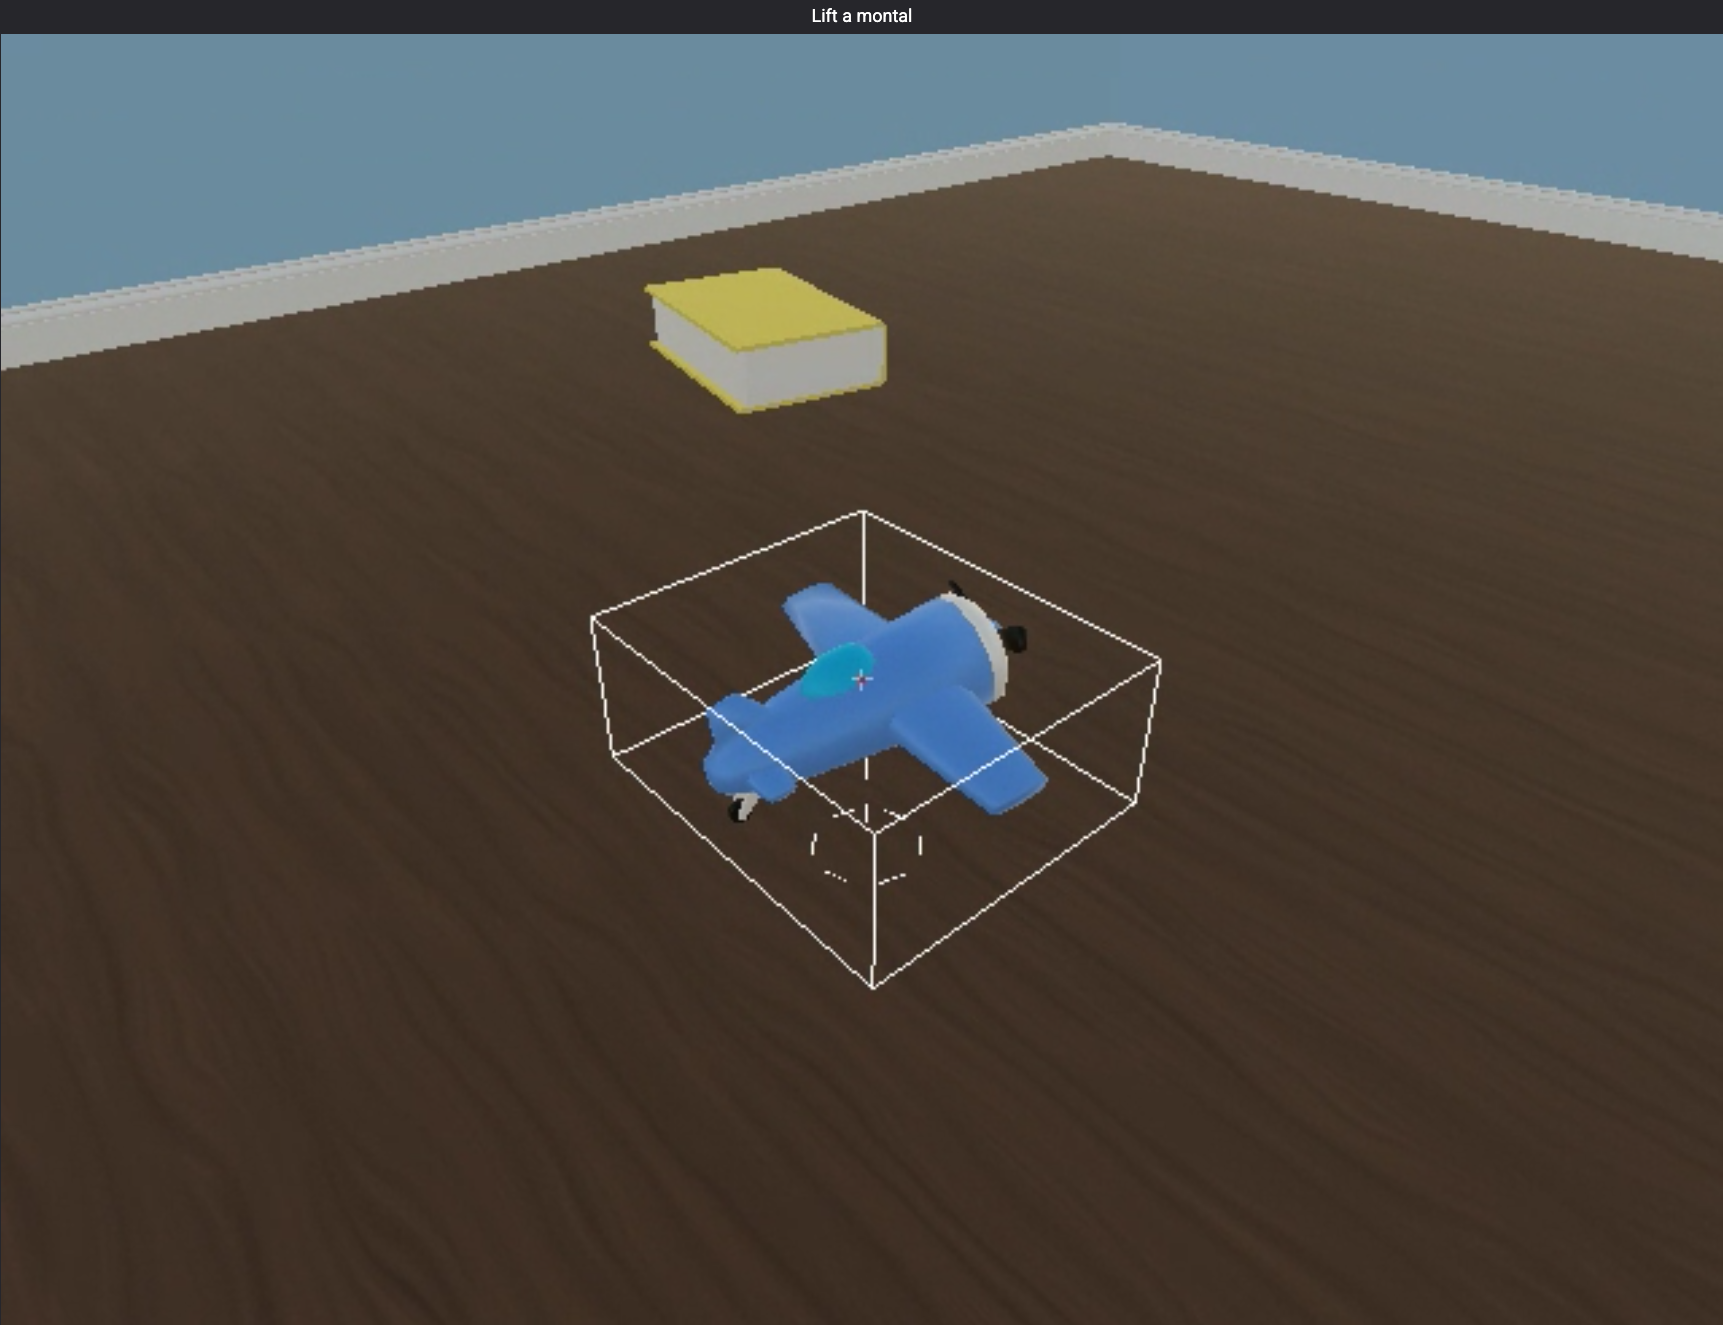
\includegraphics[width=1.5cm]{figures/task_images/fast_binding/testing.png}};
    \path [annobrace] (3.25, 0.33) -- (4.75, 0.33) node [annotext] {\footnotesize Test older word};
    
    \end{scope}
    
    \path [arrow, very thick, borange, bend right=20] (4.3, -1.1) to (0.8, 1.5);
    \path [annobrace] (4.85, -3) -- (4.85, 1.8) node [pos=0.5, anchor=center, text width=2cm, xshift=1 em,  rotate=-90] {\footnotesize \(M\) Episodes};
    \end{tikzpicture}
    }
    \vspace{-0.5em}
    \captionsetup{width=.8\textwidth}
    \caption{Recall across multiple episodes (evaluation only).} \label{fig:exp:fast_binding_tasks:episodes}
    \end{subfigure}%
